%===============
%一行目に必ず必要
%文章の形式を定義
%===============
\documentclass[dvipdfmx,a4paper]{ujarticle}% ドライバ dvipdfmx を指定する
%===============
%パッケージの定義、必要か不明
%===============
%この下4つを加えることで、mathbbが機能した
\usepackage{amsthm}
\usepackage{amsmath}
\usepackage{amssymb}
\usepackage{amsfonts}
%可換図式用パッケージ
\usepackage{amscd}
\usepackage[all]{xy}
\usepackage{tikz}
\usepackage{tikz-cd}
\usepackage{my-default}
%リンク用パッケージ
\usepackage[dvipdfmx]{hyperref}
%複数行コメント
\usetikzlibrary{shapes.geometric, arrows}
\tikzstyle{startstop} = [rectangle, rounded corners, minimum width=3cm, minimum height=1cm
\tikzstyle{io} = [trapezium, trapezium left angle=70, trapezium right angle=110, minimum width=3cm, minimum height=1cm, text centered, draw=black, fill=blue!30]
\tikzstyle{process} = [rectangle, minimum width=3cm, minimum height=1cm, text centered, draw=black, fill=orange!30]
\tikzstyle{decision} = [diamond, minimum width=3cm, minimum height=1cm, text centered, draw=black, fill=green!30]
\tikzstyle{arrow} = [thick,->,>=stealth]
\begin{document}
テスト
\begin{thm}
 基本的な結果です.
\end{thm}

\begin{tikzpicture}[domain=0:4,samples=200,>=stealth]
\draw[->] (-0.5,0) -- (4.2,0) node[right] {$x$};
\draw[->] (0,-0.5) -- (0,2.2) node[above] {$y$};
\draw plot (\x, {sqrt(\x)})
node[below] {$y=\sqrt{x}$};
\draw (0,0) node[below left] {O};
\end{tikzpicture}


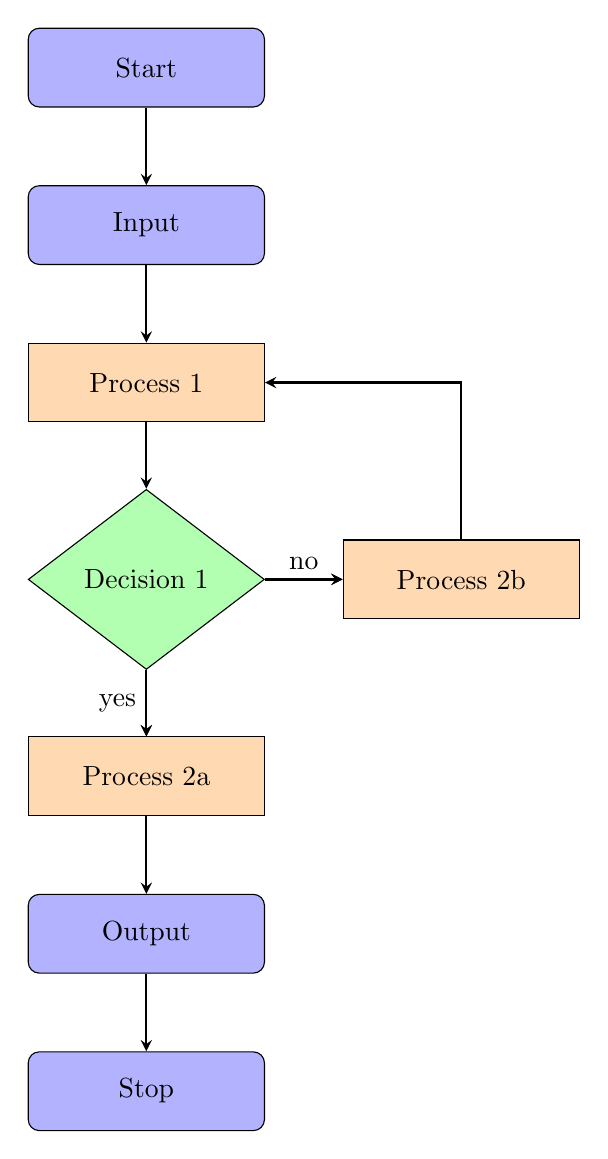
\begin{tikzpicture}[node distance=2cm]
\node (start) [startstop] {Start};
\node (in1) [startstop, below of=start] {Input};
\node (pro1) [process, below of=in1] {Process 1};
\node (dec1) [decision, below of=pro1, yshift=-0.5cm] {Decision 1};
\node (pro2a) [process, below of=dec1, yshift=-0.5cm] {Process 2a};
\node (pro2b) [process, right of=dec1, xshift=2cm] {Process 2b};
\node (out1) [startstop, below of=pro2a] {Output};
\node (stop) [startstop, below of=out1] {Stop};
\draw [arrow] (start) -- (in1);
\draw [arrow] (in1) -- (pro1);
\draw [arrow] (pro1) -- (dec1);
\draw [arrow] (dec1) -- (pro2a);
\draw [arrow] (dec1) -- (pro2b);
\draw [arrow] (dec1) -- node[anchor=east] {yes} (pro2a);
\draw [arrow] (dec1) -- node[anchor=south] {no} (pro2b);
\draw [arrow] (pro2b) |- (pro1);
\draw [arrow] (pro2a) -- (out1);
\draw [arrow] (out1) -- (stop);
\end{tikzpicture}

\end{document}
